\documentclass[11pt,a4paper]{article}
\usepackage[margin=2.4cm]{geometry}
\usepackage[T1]{fontenc}
\usepackage{lmodern}
\usepackage[letterspace=180]{microtype}
\usepackage{booktabs}
\usepackage{amsmath,amssymb}
\usepackage{parskip}
\usepackage{xcolor}
\usepackage[most]{tcolorbox}
\usepackage{titlesec}
\usepackage{caption}
\usepackage{graphicx}
\usepackage{enumitem}
\usepackage{eurosym}
\usepackage{tikz}
\usetikzlibrary{positioning,arrows.meta,shapes.misc}

\definecolor{bcnavy}{RGB}{24,38,68}
\definecolor{bcgold}{RGB}{198,160,74}
\definecolor{bcteal}{RGB}{23,110,120}
\definecolor{bcgrey}{RGB}{95,95,95}
\definecolor{bcred}{RGB}{160,60,50}

\titleformat{\section}{\bfseries\large\color{bcnavy}}{\thesection.}{0.6em}{}
\titleformat{\subsection}{\bfseries\color{bcteal}}{}{0em}{}
\captionsetup{font={footnotesize},labelformat=empty,textfont={color=bcgrey}}
\newcommand{\tabnote}[1]{\begin{center}\begin{minipage}{0.92\textwidth}
  \footnotesize\color{bcgrey}#1\end{minipage}\end{center}}

\tikzset{
  ent/.style={draw=bcnavy, thick, fill=bcnavy!4, rounded corners=2pt,
              align=center, minimum height=0.9cm, inner sep=5pt,
              font=\footnotesize},
  fam/.style={ent, fill=bcgold!12, draw=bcgold!80!black},
  inv/.style={ent, fill=bcteal!8, draw=bcteal},
  reg/.style={ent, fill=bcred!6, draw=bcred, dashed},
  mkt/.style={ent, fill=white, draw=bcgrey},
  flow/.style={-{Stealth[length=2.4mm]}, thick, color=bcnavy},
  ret/.style={-{Stealth[length=2.4mm]}, thick, dashed, color=bcteal},
  lbl/.style={font=\scriptsize\itshape, color=bcgrey, align=center},
}

\begin{document}

% ---------------------------------------------------------------- header
\begin{center}
{\Large\bfseries\color{bcnavy} Third-Party Capital --- Structural Options}\\[0.15cm]
{\color{bcnavy} four routes to outside investors, with the regulation that actually applies}\\[0.25cm]
{\small\color{bcgrey} Bayesian Capital --- internal, strictly confidential
\;$\bullet$\; 16 September 2026 \;$\bullet$\; prepared for discussion with Irish counsel}
\end{center}
\vspace{0.1cm}
{\color{bcnavy}\hrule height 0.8pt}
\vspace{0.3cm}

\begin{tcolorbox}[colback=bcred!5, colframe=bcred, boxrule=0.8pt]
\footnotesize\textbf{This note is not legal or tax advice.} It is a structured
briefing for a meeting with an Irish funds/financial-regulation solicitor,
prepared from internal discussion. Thresholds, processes and tax treatments
stated here are as generally understood and must be confirmed as current by
counsel before anything is signed or any money moves.
\end{tcolorbox}

\section{The question, and the regulation that actually applies}

Bayesian Capital (``BC'') is a family-owned Irish company running a
systematic nine-name book. The principal is considering admitting third-party
investors, with no appetite for authorisation as an investment adviser. Two
structures were originally proposed: an SPV subsidiary of BC, or a new
company licensing the BC system --- each run for a defined period and wound up
by members' voluntary liquidation (MVL) to return capital.

\textbf{The key reframing: adviser regulation (MiFID) was never the main
exposure --- fund regulation (AIFMD) is.} Under the Irish AIFMD regulations,
an entity that (i) raises capital from a number of investors, (ii) to invest
under a defined investment policy, (iii) for those investors' benefit, is an
\emph{Alternative Investment Fund}, whatever its legal wrapper --- and whoever
performs its portfolio management is its \emph{AIFM}. Both original proposals
are caught equally: the MVL end-date does not help (closed-ended AIFs are
still AIFs), and a licence agreement does not change who manages --- if the
principal runs the morning scripts, the principal is the manager. The Central
Bank reads substance, not form. BC today is out of scope only because it is a
\textbf{family office}, expressly outside AIFMD; the first euro of genuinely
third-party capital is what changes the analysis, not the wrapper it arrives
in.

\subsection{Status quo, for reference}

\begin{center}
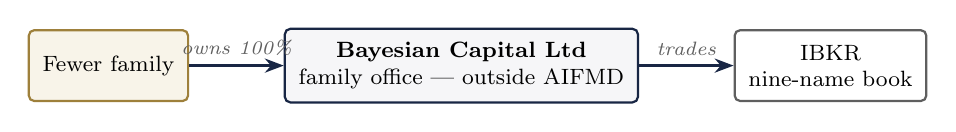
\begin{tikzpicture}[node distance=0.55cm and 1.2cm]
\node[fam] (fam) {Fewer family};
\node[ent, right=of fam] (bc) {\textbf{Bayesian Capital Ltd}\\family office --- outside AIFMD};
\node[mkt, right=of bc] (ib) {IBKR\\nine-name book};
\draw[flow] (fam) -- node[lbl, above]{owns 100\%} (bc);
\draw[flow] (bc) -- node[lbl, above]{trades} (ib);
\end{tikzpicture}
\end{center}

\section{Option A --- SPV subsidiary of BC \hfill
  {\normalsize\color{bcred} not recommended}}

\begin{center}
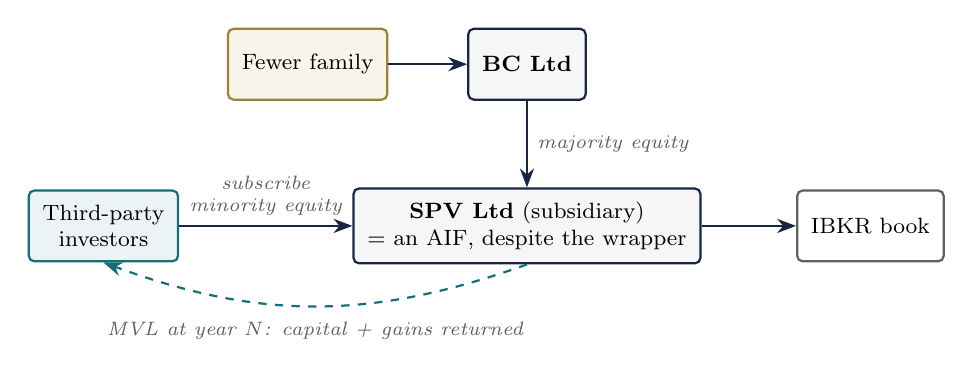
\begin{tikzpicture}[node distance=0.55cm and 1.0cm]
\node[fam] (fam) {Fewer family};
\node[ent, right=of fam] (bc) {\textbf{BC Ltd}};
\node[ent, below=1.1cm of bc] (spv) {\textbf{SPV Ltd} (subsidiary)\\= an AIF, despite the wrapper};
\node[inv, left=2.2cm of spv] (inv) {Third-party\\investors};
\node[mkt, right=1.2cm of spv] (ib) {IBKR book};
\draw[flow] (fam) -- (bc);
\draw[flow] (bc) -- node[lbl, right]{majority equity} (spv);
\draw[flow] (inv) -- node[lbl, above]{subscribe\\minority equity} (spv);
\draw[flow] (spv) -- (ib);
\draw[ret] (spv.south) to[bend left=20]
  node[lbl, below=2pt]{MVL at year $N$: capital + gains returned} (inv.south);
\end{tikzpicture}
\end{center}

Same AIFMD analysis as every other option --- and it adds problems the others
avoid: outside investors become \textbf{minority shareholders inside the
family group}, bringing statutory oppression-remedy rights, pre-emption and
exit expectations into BC's perimeter; the SPV consolidates into the family
company; and any failure travels up reputationally and possibly legally. The
corporate separation the structure appears to offer is weakest exactly where
it is wanted.

\section{Option B --- NewCo vehicle + system licence + registered AIFM \hfill
  {\normalsize\color{bcteal} the recommended shape}}

\begin{center}
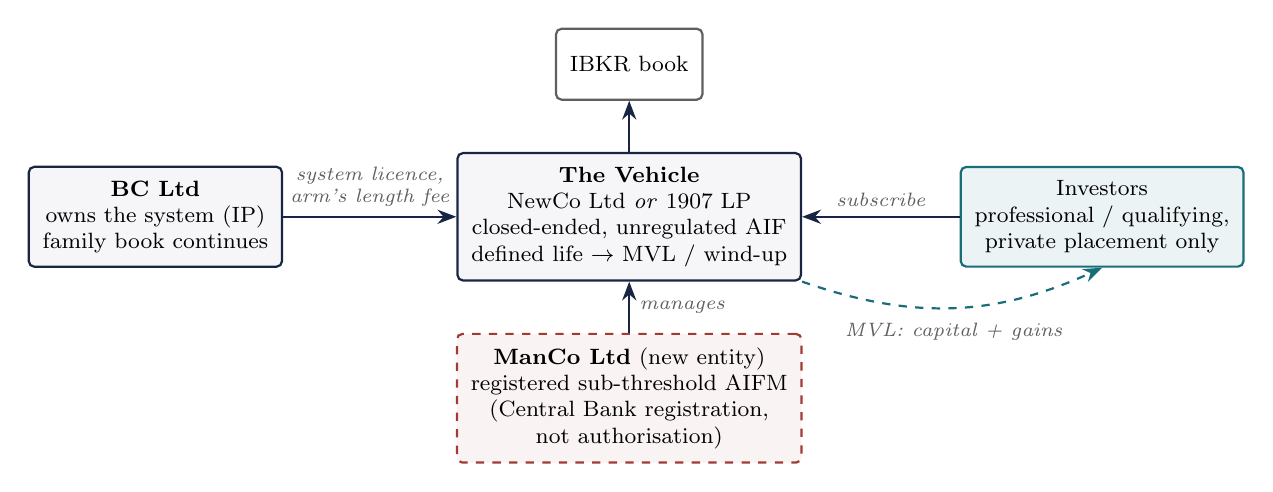
\begin{tikzpicture}[node distance=0.65cm and 0.9cm]
\node[ent] (bc) {\textbf{BC Ltd}\\owns the system (IP)\\family book continues};
\node[ent, right=2.2cm of bc] (veh) {\textbf{The Vehicle}\\NewCo Ltd \emph{or} 1907 LP\\closed-ended, unregulated AIF\\defined life $\to$ MVL / wind-up};
\node[inv, right=2.0cm of veh] (inv) {Investors\\professional / qualifying,\\private placement only};
\node[reg, below=of veh] (manco) {\textbf{ManCo Ltd} (new entity)\\registered sub-threshold AIFM\\(Central Bank registration,\\not authorisation)};
\node[mkt, above=of veh] (ib) {IBKR book};
\draw[flow] (bc) -- node[lbl, above]{system licence,\\arm's length fee} (veh);
\draw[flow] (inv) -- node[lbl, above]{subscribe} (veh);
\draw[flow] (manco) -- node[lbl, right]{manages} (veh);
\draw[flow] (veh) -- (ib);
\draw[ret] (veh.south east) to[bend right=22]
  node[lbl, below=2pt]{MVL: capital + gains} (inv.south);
\end{tikzpicture}
\end{center}

Accepts the AIF analysis and takes the cheapest compliant status in European
fund management. Key design choices:

\begin{itemize}[leftmargin=1.6em, itemsep=2pt]
\item \textbf{External ManCo, and a new one} --- not BC. Registering BC would
      put the family company inside the regulatory perimeter; a separate
      ManCo registers once and manages successive vintages (vintage II is a
      notification, not a new registration).
\item \textbf{Vehicle form is a first-meeting tax question.} A plain Irish
      company pays corporation tax inside the vehicle (share-dealing
      treatment, close-company surcharge questions); the favourable fund tax
      regime belongs to \emph{regulated} funds, deliberately not created
      here. The classic sub-threshold answer is a \textbf{1907 limited
      partnership} --- tax-transparent, investors taxed at their own rates,
      ManCo as general partner. Which wins depends on the investors' tax
      positions and materially changes net returns.
\item \textbf{The licence is a related-party transaction}: arm's-length
      pricing, VAT treatment, and close-company surcharge on passive licence
      income in BC all need counsel/accountant sign-off.
\item \textbf{US plumbing}: W-8BEN-E for the vehicle, treaty withholding on
      any dividends --- mechanical, but owned by someone.
\end{itemize}

\section{Option C --- a genuine co-venture, outside AIFMD \hfill
  {\normalsize\color{bcgrey} thin ice, fact-specific}}

\begin{center}
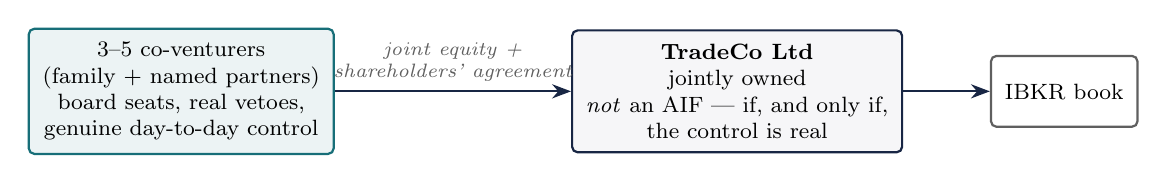
\begin{tikzpicture}[node distance=0.55cm and 1.1cm]
\node[inv] (cov) {3--5 co-venturers\\(family + named partners)\\board seats, real vetoes,\\genuine day-to-day control};
\node[ent, right=3.0cm of cov] (tc) {\textbf{TradeCo Ltd}\\jointly owned\\\emph{not} an AIF --- if, and only if,\\the control is real};
\node[mkt, right=of tc] (ib) {IBKR book};
\draw[flow] (cov) -- node[lbl, above]{joint equity +\\shareholders' agreement} (tc);
\draw[flow] (tc) -- (ib);
\end{tikzpicture}
\end{center}

The AIF definition requires ``raising capital from a number of investors'';
a genuine joint venture whose participants exercise real ongoing control can
fall outside it. That requires the control to be true in fact --- board
participation, strategy approval through the gates process, not passive
cheques with decorative titles. This is the highest-value question to put to
counsel, and the structure most likely to be re-characterised if the
substance is thin.

\section{Option D --- fixed-coupon loan notes into BC \hfill
  {\normalsize\color{bcgrey} different economics entirely}}

\begin{center}
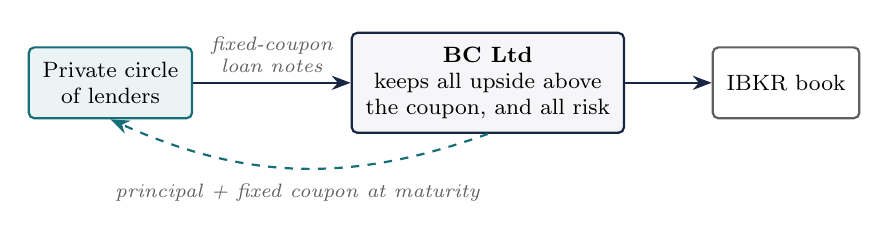
\begin{tikzpicture}[node distance=0.55cm and 1.1cm]
\node[inv] (ln) {Private circle\\of lenders};
\node[ent, right=2.0cm of ln] (bc) {\textbf{BC Ltd}\\keeps all upside above\\the coupon, and all risk};
\node[mkt, right=of bc] (ib) {IBKR book};
\draw[flow] (ln) -- node[lbl, above]{fixed-coupon\\loan notes} (bc);
\draw[flow] (bc) -- (ib);
\draw[ret] (bc.south) to[bend left=22]
  node[lbl, below=2pt]{principal + fixed coupon at maturity} (ln.south);
\end{tikzpicture}
\end{center}

No fund, no AIF, near-zero regulatory surface --- because the investors are
lenders, not participants. Constraints: the coupon must be genuinely fixed
(profit participation drifts back toward the fund analysis), and the circle
genuinely private and identified (borrowing ``from the public'' drifts toward
deposit-taking rules). Economically unlike the proposal: lenders cap their
upside; BC gears its own equity.

\section{Sub-threshold (registered) AIFM --- what Option B's status involves}

\begin{itemize}[leftmargin=1.6em, itemsep=2pt]
\item \textbf{Eligibility}: AUM $\leq$ \euro 100m, or $\leq$ \euro 500m where
      unleveraged and closed-ended with no redemption rights for five years
      --- the MVL design is exactly the \euro 500m category, passed by two
      orders of magnitude.
\item \textbf{The registration}: a Central Bank portal filing --- identity of
      the AIFM, its directors and beneficial owners, the AIF(s), the
      investment strategies. Registration, not authorisation: no minimum
      regulatory capital, no depositary, no programme-of-activity approval.
      Typically weeks; the Bank's own fee negligible. Realistic all-in cost
      for the full structure (vehicle, PPM, subscription and shareholders'
      documents, registration) $\approx$ \euro 15--30k, dominated by legal
      drafting that any version of taking outside money requires anyway.
\item \textbf{Ongoing}: an annual cut-down Annex IV report (AUM, main
      instruments, principal exposures, concentrations --- an afternoon for a
      nine-name book); documented threshold monitoring; material-change
      notifications; plus the plumbing any vehicle owes regardless ---
      AML/CFT with a named MLRO, beneficial-ownership register, FATCA/CRS,
      audited accounts.
\item \textbf{What it does not give}: no EU marketing passport (national
      private placement only) and, practically, \textbf{no retail investors}
      --- the vehicle stays an unregulated AIF, placed privately with
      professional or genuinely sophisticated investors whose documents say
      in plain words that no regulator has reviewed the fund.
\end{itemize}

\section{Cross-cutting pitfalls (every option)}

\begin{itemize}[leftmargin=1.6em, itemsep=2pt]
\item \textbf{The allocation conflict} --- the first question investors'
      advisers will ask: the family book and the investor vehicle would run
      the same signals through the same broker. A written allocation policy
      (aggregated orders split pro-rata by capital) must exist before the
      first overlapping bid.
\item \textbf{Performance representations}: once outside money reads the plan
      numbers, they are owned. The investor pack must carry the cold-state
      framing --- the plan band, the unprotected 2022 replay, the measured
      drawdown --- as prominently as the upside.
\item \textbf{MVL lock-in mechanics}: closed-ended means no redemption valve;
      the shareholders' or partnership agreement needs answers for an
      investor's death, divorce or distress mid-life.
\item \textbf{Key-man}: the machine is one principal and part-time analysts;
      third-party capital turns ``what if the principal is unavailable''
      into a contractual question.
\item \textbf{Offer mechanics}: an Irish private company cannot offer
      securities to the public --- any raise stays a genuine private
      placement to a small, identified circle.
\end{itemize}

\section{Comparison}

\begin{center}
\footnotesize
\begin{tabular}{@{}p{2.5cm}p{2.9cm}p{3.1cm}p{3.0cm}p{2.9cm}@{}}
\toprule
 & \textbf{A: SPV sub} & \textbf{B: NewCo + licence} & \textbf{C: co-venture} & \textbf{D: loan notes} \\
\midrule
AIFMD status      & AIF (caught)          & AIF; registered AIFM      & outside --- if real       & not a fund \\
Regulatory burden & same as B, no gain    & light (registration)      & none --- if it holds      & near zero \\
Separation from BC & \textbf{poor}        & good (firewalled)         & good                      & none (BC borrows) \\
Investor economics & equity, pooled       & equity, pooled            & equity, joint             & fixed coupon \\
Tax shape         & group complications   & LP transparency available & company                   & interest \\
Fragility         & minority rights inside the group & ---            & re-characterisation risk  & drift to deposits / profit-share \\
Verdict           & {\color{bcred}avoid}  & {\color{bcteal}\textbf{recommended shape}} & explore with counsel & if lender economics suit \\
\bottomrule
\end{tabular}
\end{center}

\section{For the solicitor meeting}

\textbf{Decisions to bring}: expected investor count and profile
(professional?), target size, intended life, whether the family book
continues alongside (it does --- hence the allocation policy), appetite for
the co-venture governance give-up.

\textbf{Questions to ask}: (1) company vs 1907 LP for the vehicle, given
these investors' tax positions; (2) can our specific circle be structured as
a genuine non-AIF co-venture, and what substance would it need to survive
re-characterisation; (3) registered-AIFM scope --- internally managed vs
external ManCo for a vintage series; (4) licence pricing/VAT/surcharge
treatment for BC; (5) MVL tax treatment for investors (capital vs income,
and any anti-avoidance exposure); (6) the private-placement boundaries for
the raise; (7) AML/MLRO arrangements proportionate to a vehicle this size.

\vspace{0.4cm}
{\color{bcnavy}\hrule height 0.8pt}
\vspace{0.2cm}
{\footnotesize\color{bcgrey} Prepared from the internal structuring
discussion of 7--8 September 2026. Not legal or tax advice; all regulatory
and tax statements to be confirmed as current by counsel.}

\end{document}
